% Neural Networks Primer: Teaching Computers to Recognize Your Handwriting
% Complete 55-Slide Version for BSc Students (No Prerequisites)
% Following the comprehensive content improvement plan
\documentclass[8pt,aspectratio=169]{beamer}
\usetheme{Madrid}
\usecolortheme{seahorse}

% Color definitions - minimalist style
\definecolor{mainGray}{RGB}{64,64,64}
\definecolor{accentGray}{RGB}{180,180,180}
\definecolor{lightGray}{RGB}{240,240,240}
\definecolor{highlightRed}{RGB}{220,50,50}
\definecolor{learnGreen}{RGB}{50,180,50}
\definecolor{deepBlue}{RGB}{74,144,226}

\setbeamercolor{structure}{fg=mainGray}
\setbeamercolor{normal text}{fg=mainGray}
\setbeamertemplate{navigation symbols}{}

% Commands
\newcommand{\highlight}[1]{{\color{highlightRed}#1}}
\newcommand{\secondary}[1]{{\color{accentGray}#1}}
\newcommand{\success}[1]{{\color{learnGreen}#1}}
\newcommand{\concept}[1]{{\color{deepBlue}#1}}

\usepackage{tikz}
\usepackage{amsmath}
\usepackage{amssymb}
\usepackage{listings}
\usepackage{graphicx}

\title{Teaching Computers to Recognize Your Handwriting}
\subtitle{A Complete Journey from Simple Rules to Deep Learning}
\author{NLP Course 2025}
\date{}

\begin{document}

% Title Slide
\begin{frame}
\titlepage
\vfill
\begin{center}
\secondary{\small From impossible rules to learning machines: A complete journey anyone can understand}
\end{center}
\end{frame}

% ==========================================
% PART 1: OPENING PROBLEM (Slides 1-5)
% ==========================================

% Slide 1: Your Handwriting is Unique
\begin{frame}{Slide 1: Your Handwriting is Unique}
\begin{center}
{\Large \textbf{Everyone writes the letter "A" differently}}
\end{center}
\vspace{5mm}
\begin{columns}
\column{0.6\textwidth}
\begin{center}
\includegraphics[width=\textwidth]{../figures/handwriting_variations.pdf}
\end{center}

\column{0.38\textwidth}
\textbf{You recognize them all because:}
\begin{itemize}
\item You learned from examples
\item You see the pattern, not exact shape
\item Your brain generalizes
\end{itemize}

\vspace{5mm}
\textbf{But a computer sees:}
\begin{itemize}
\item Just pixels (dots)
\item No inherent meaning
\item Needs exact instructions
\end{itemize}
\end{columns}
\vfill
\secondary{\footnotesize This is the fundamental challenge: How do we teach a machine to see patterns like we do?}
\end{frame}

% Slide 2: The Challenge
\begin{frame}{Slide 2: The Challenge}
\begin{center}
{\Large \textbf{Computers Need Rules, But Writing is Infinite}}
\end{center}
\vspace{5mm}
\begin{columns}
\column{0.48\textwidth}
\textbf{The Variety Problem:}
\begin{itemize}
\item Print vs cursive
\item Size variations
\item Rotation angles
\item Thickness differences
\item Personal style
\item Speed of writing
\item Writing instrument
\end{itemize}

\column{0.48\textwidth}
\textbf{The Numbers:}
\begin{itemize}
\item 7 billion people
\item Each writes uniquely
\item Changes with mood/age
\item = Infinite variations!
\end{itemize}

\vspace{5mm}
\begin{center}
\fbox{\parbox{0.9\textwidth}{
\centering
\highlight{Central Question:}\\
How can we possibly program\\
rules for infinite variations?
}}
\end{center}
\end{columns}
\vfill
\secondary{\footnotesize Spoiler: We can't. We need a different approach entirely.}
\end{frame}

% Slide 3: Traditional Programming Fails
\begin{frame}[fragile]{Slide 3: Traditional Programming Fails}
\begin{center}
{\Large \textbf{Why IF-THEN Rules Don't Work}}
\end{center}
\vspace{5mm}
\begin{columns}
\column{0.5\textwidth}
\textbf{Attempt at Programming "A" Recognition:}
\begin{lstlisting}[basicstyle=\tiny, language=Python]
def recognize_A(pixels):
    if has_triangle_top(pixels):
        if has_horizontal_bar(pixels):
            if two_diagonal_lines(pixels):
                return "It's an A!"

    # But wait...
    if cursive_style(pixels):
        # Different rules!

    if child_handwriting(pixels):
        # More different rules!

    # This goes on forever...
\end{lstlisting}

\column{0.48\textwidth}
\begin{center}
\includegraphics[width=0.9\textwidth]{../figures/rules_vs_learning.pdf}
\end{center}

\textbf{Why This Fails:}
\begin{itemize}
\item Can't anticipate all styles
\item Rules conflict with each other
\item Exceptions have exceptions
\item \highlight{Impossible to maintain!}
\end{itemize}
\end{columns}
\vfill
\secondary{\footnotesize After decades of trying, programmers gave up on rule-based recognition}
\end{frame}

% Slide 4: Nature's Solution
\begin{frame}{Slide 4: Nature's Solution - How Children Learn}
\begin{center}
{\Large \textbf{Children Don't Use Rules}}
\end{center}
\vspace{5mm}
\begin{columns}
\column{0.48\textwidth}
\textbf{A Child Learning to Read:}
\begin{enumerate}
\item Sees letter "A" in a book
\item Parent says "That's an A"
\item Sees different "A" styles
\item Makes mistakes
\item Gets corrected
\item Brain adjusts understanding
\item Eventually recognizes any "A"
\end{enumerate}

\vspace{3mm}
\success{No rules memorized!}\\
\success{Pattern discovered naturally!}

\column{0.48\textwidth}
\textbf{The Learning Process:}
\begin{center}
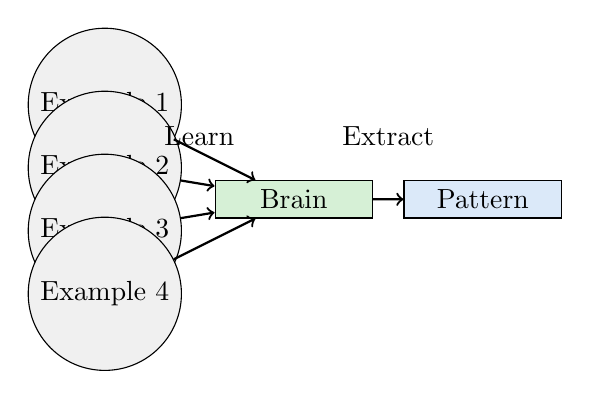
\begin{tikzpicture}[scale=0.8]
\node[circle,draw,fill=lightGray] (ex1) at (0,3) {Example 1};
\node[circle,draw,fill=lightGray] (ex2) at (0,2) {Example 2};
\node[circle,draw,fill=lightGray] (ex3) at (0,1) {Example 3};
\node[circle,draw,fill=lightGray] (ex4) at (0,0) {Example 4};

\node[rectangle,draw,fill=learnGreen!20,minimum width=2cm] (brain) at (3,1.5) {Brain};
\node[rectangle,draw,fill=deepBlue!20,minimum width=2cm] (pattern) at (6,1.5) {Pattern};

\draw[->,thick] (ex1) -- (brain);
\draw[->,thick] (ex2) -- (brain);
\draw[->,thick] (ex3) -- (brain);
\draw[->,thick] (ex4) -- (brain);
\draw[->,thick] (brain) -- (pattern);

\node at (1.5,2.5) {Learn};
\node at (4.5,2.5) {Extract};
\end{tikzpicture}
\end{center}

\textbf{Key Insight:}\\
Learning from examples works\\
better than following rules!
\end{columns}
\vfill
\secondary{\footnotesize This biological inspiration would revolutionize computing}
\end{frame}

% Slide 5: The Big Idea
\begin{frame}{Slide 5: The Big Idea}
\begin{center}
{\Large \textbf{What if Computers Could Learn Like Children?}}
\end{center}
\vspace{5mm}
\begin{columns}
\column{0.5\textwidth}
\textbf{Traditional Programming:}
\begin{itemize}
\item Human writes rules
\item Computer follows rules
\item Fails on new situations
\item Needs constant updates
\end{itemize}

\vspace{5mm}
\textbf{Machine Learning:}
\begin{itemize}
\item Show many examples
\item Computer finds patterns
\item Generalizes to new cases
\item Improves with more data
\end{itemize}

\column{0.5\textwidth}
\begin{center}
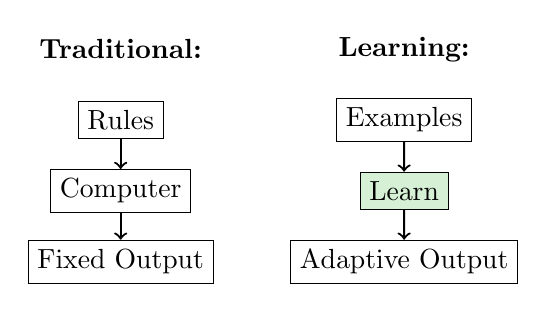
\begin{tikzpicture}[scale=0.9]
% Traditional
\node at (0,3.5) {\textbf{Traditional:}};
\node[rectangle,draw] (rules) at (0,2.5) {Rules};
\node[rectangle,draw] (computer1) at (0,1.5) {Computer};
\node[rectangle,draw] (output1) at (0,0.5) {Fixed Output};
\draw[->,thick] (rules) -- (computer1);
\draw[->,thick] (computer1) -- (output1);

% Machine Learning
\node at (4,3.5) {\textbf{Learning:}};
\node[rectangle,draw] (examples) at (4,2.5) {Examples};
\node[rectangle,draw,fill=learnGreen!20] (computer2) at (4,1.5) {Learn};
\node[rectangle,draw] (output2) at (4,0.5) {Adaptive Output};
\draw[->,thick] (examples) -- (computer2);
\draw[->,thick] (computer2) -- (output2);
\end{tikzpicture}
\end{center}

\vspace{5mm}
\begin{center}
\fbox{\parbox{0.9\textwidth}{
\centering
\concept{\textbf{The Revolution:}}\\
Instead of programming HOW,\\
we show examples of WHAT
}}
\end{center}
\end{columns}
\vfill
\secondary{\footnotesize This idea, proposed in 1957, would take 60 years to fully realize}
\end{frame}

% ==========================================
% PART 2: BUILDING THE FIRST NEURON (Slides 6-15)
% ==========================================

% Slide 6: A Neuron is a Decision Maker
\begin{frame}{Slide 6: A Neuron is a Decision Maker}
\begin{center}
{\Large \textbf{Think of a Neuron Like a Traffic Light}}
\end{center}
\vspace{5mm}
\begin{columns}
\column{0.5\textwidth}
\textbf{Traffic Light Decision:}
\begin{itemize}
\item Input 1: Cars waiting?
\item Input 2: Pedestrian button?
\item Input 3: Time since last change?
\item Decision: Change light or not
\end{itemize}

\vspace{5mm}
\textbf{Neuron Decision:}
\begin{itemize}
\item Input 1: Pixel 1 value
\item Input 2: Pixel 2 value
\item Input 3: Pixel 3 value
\item Decision: Is it an "A" or not
\end{itemize}

\column{0.5\textwidth}
\begin{center}
\includegraphics[width=\textwidth]{../figures/neuron_as_voter.pdf}
\end{center}

\textbf{The Process:}
\begin{enumerate}
\item Receive inputs
\item Weight their importance
\item Add them up
\item Make decision
\end{enumerate}
\end{columns}
\vfill
\secondary{\footnotesize A neuron is just a weighted voter - nothing magical!}
\end{frame}

% Slide 7: Everything is Numbers
\begin{frame}{Slide 7: Everything Must Become Numbers}
\begin{center}
{\Large \textbf{From Handwriting to Numbers}}
\end{center}
\vspace{5mm}
\begin{columns}
\column{0.6\textwidth}
\begin{center}
\includegraphics[width=\textwidth]{../figures/pixel_to_numbers.pdf}
\end{center}

\column{0.38\textwidth}
\textbf{The Transformation:}
\begin{enumerate}
\item Scan the letter
\item Divide into grid (pixels)
\item Black pixel = 1
\item White pixel = 0
\item Now we have numbers!
\end{enumerate}

\vspace{5mm}
\textbf{Example (5×5 grid):}
\begin{itemize}
\item Center top: 1 (black)
\item Sides: mostly 0 (white)
\item Total: 25 numbers
\item Computer can process!
\end{itemize}
\end{columns}
\vfill
\secondary{\footnotesize Everything in AI starts with converting the real world into numbers}
\end{frame}

% Slide 8: Weights are Importance Scores
\begin{frame}{Slide 8: Weights are Importance Scores}
\begin{center}
{\Large \textbf{Not All Pixels Are Equally Important}}
\end{center}
\vspace{5mm}
\begin{columns}
\column{0.48\textwidth}
\textbf{Voting Analogy:}
\begin{itemize}
\item Expert vote: Weight = 10
\item Regular vote: Weight = 1
\item Novice vote: Weight = 0.1
\end{itemize}

\vspace{5mm}
\textbf{For Letter "A":}
\begin{itemize}
\item Top center pixel: High weight
\item Middle sides: High weight
\item Bottom corners: Low weight
\item Very bottom: Negative weight
\end{itemize}

\column{0.48\textwidth}
\begin{center}
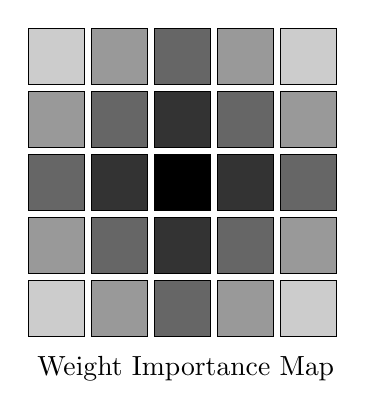
\begin{tikzpicture}[scale=0.8]
% Grid showing weight importance
\foreach \x in {0,...,4}
\foreach \y in {0,...,4}
{
    \pgfmathtruncatemacro{\gray}{100 - abs(\x-2)*20 - abs(\y-2)*20}
    \fill[black!\gray] (\x,\y) rectangle (\x+0.9,\y+0.9);
    \draw (\x,\y) rectangle (\x+0.9,\y+0.9);
}
\node at (2.5,-0.5) {Weight Importance Map};
\end{tikzpicture}
\end{center}

\textbf{Learning = Finding Right Weights:}
\begin{itemize}
\item Start with random weights
\item See examples
\item Adjust weights
\item Improve recognition
\end{itemize}
\end{columns}
\vfill
\secondary{\footnotesize The entire learning process is just finding the right importance scores}
\end{frame}

% Slide 9: Adding It All Up
\begin{frame}{Slide 9: Adding It All Up (No Algebra Needed!)}
\begin{center}
{\Large \textbf{Simple Math: Multiply and Add}}
\end{center}
\vspace{5mm}
\begin{columns}
\column{0.5\textwidth}
\textbf{Concrete Example:}
\begin{center}
\begin{tabular}{|l|c|c|c|}
\hline
\textbf{Pixel} & \textbf{Value} & \textbf{Weight} & \textbf{Result} \\
\hline
Top center & 1 & ×3 & = 3 \\
Left middle & 1 & ×2 & = 2 \\
Right middle & 1 & ×2 & = 2 \\
Bottom center & 0 & ×(-1) & = 0 \\
\hline
\multicolumn{3}{|r|}{\textbf{Total:}} & \textbf{7} \\
\hline
\end{tabular}
\end{center}

\vspace{3mm}
It's just like calculating a bill:
\begin{itemize}
\item 1 pizza × \$10 = \$10
\item 2 sodas × \$3 = \$6
\item Total = \$16
\end{itemize}

\column{0.48\textwidth}
\textbf{What the Neuron Does:}
\begin{enumerate}
\item Takes each input (0 or 1)
\item Multiplies by its weight
\item Adds all results
\item Gets a total score
\end{enumerate}

\vspace{5mm}
\begin{center}
\fbox{\parbox{0.9\textwidth}{
\centering
\textbf{The Formula:}\\
Total = (Input1 × Weight1) +\\
(Input2 × Weight2) + ...
}}
\end{center}

\vspace{3mm}
\success{That's it! No complex math!}
\end{columns}
\vfill
\secondary{\footnotesize This simple operation, repeated millions of times, powers all of AI}
\end{frame}

% Slide 10: Making the Decision
\begin{frame}{Slide 10: Making the Decision}
\begin{center}
{\Large \textbf{Is the Total High Enough?}}
\end{center}
\vspace{5mm}
\begin{columns}
\column{0.48\textwidth}
\textbf{Setting a Threshold:}
\begin{itemize}
\item Total score: 7
\item Threshold: 5
\item Is 7 > 5? \success{Yes!}
\item Decision: "It's an A!"
\end{itemize}

\vspace{5mm}
\textbf{Like a Scale:}
\begin{center}
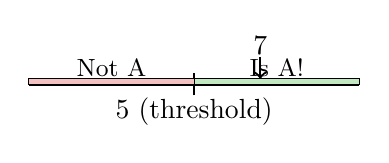
\begin{tikzpicture}[scale=0.7]
% Draw scale
\draw[thick] (0,0) -- (6,0);
\draw[thick] (3,-0.2) -- (3,0.2);
\node at (3,-0.5) {5 (threshold)};

% Draw pointer
\draw[thick,->] (4.2,0.5) -- (4.2,0.1);
\node at (4.2,0.7) {7};

% Labels
\node at (1.5,0.3) {\small Not A};
\node at (4.5,0.3) {\small Is A!};

\draw[fill=highlightRed!30] (0,0) rectangle (3,0.1);
\draw[fill=learnGreen!30] (3,0) rectangle (6,0.1);
\end{tikzpicture}
\end{center}

\column{0.48\textwidth}
\textbf{Different Thresholds:}
\begin{itemize}
\item Low threshold: More "yes"
\item High threshold: More "no"
\item Just right: Good accuracy
\end{itemize}

\vspace{5mm}
\textbf{Real Examples:}
\begin{itemize}
\item Email spam filter: Threshold = 0.8
\item Medical diagnosis: Threshold = 0.95
\item Face unlock: Threshold = 0.7
\end{itemize}

\vspace{3mm}
\highlight{Threshold is also learned!}
\end{columns}
\vfill
\secondary{\footnotesize The threshold determines how confident the neuron needs to be}
\end{frame}

% Slide 11: Learning from Mistakes
\begin{frame}{Slide 11: Learning from Mistakes}
\begin{center}
{\Large \textbf{Wrong Answer? Adjust the Weights!}}
\end{center}
\vspace{5mm}
\begin{columns}
\column{0.55\textwidth}
\begin{center}
\includegraphics[width=\textwidth]{../figures/weight_adjustment_visual.pdf}
\end{center}

\column{0.43\textwidth}
\textbf{The Learning Rule:}
\begin{enumerate}
\item Show an example
\item Neuron makes prediction
\item Check if correct
\item If wrong: adjust weights
\item Repeat many times
\end{enumerate}

\vspace{5mm}
\textbf{How to Adjust:}
\begin{itemize}
\item Pixel was 1, answer wrong?\\
  → Increase its weight
\item Pixel was 0, answer wrong?\\
  → Decrease its weight
\item Answer correct?\\
  → Keep weights same
\end{itemize}
\end{columns}
\vfill
\secondary{\footnotesize This is exactly how children learn - through trial and error}
\end{frame}

% Slide 12: Watching It Learn
\begin{frame}{Slide 12: Watching a Neuron Learn}
\begin{center}
{\Large \textbf{5 Training Steps with Real Numbers}}
\end{center}
\vspace{3mm}
\begin{center}
\includegraphics[width=0.95\textwidth]{../figures/training_steps_numbered.pdf}
\end{center}

\begin{columns}
\column{0.48\textwidth}
\textbf{Step by Step:}
\begin{itemize}
\item Step 1: Random weights, 20\% correct
\item Step 2: Small adjustments, 35\% correct
\item Step 3: Pattern emerging, 60\% correct
\item Step 4: Almost there, 85\% correct
\item Step 5: Trained! 95\% correct
\end{itemize}

\column{0.48\textwidth}
\textbf{What's Happening:}
\begin{itemize}
\item Weights organize themselves
\item Important pixels get high weights
\item Unimportant get low weights
\item Pattern detector emerges
\item \success{No programming required!}
\end{itemize}
\end{columns}
\vfill
\secondary{\footnotesize After seeing hundreds of examples, the neuron "knows" what an A looks like}
\end{frame}

% Slide 13: Success on Simple Problems
\begin{frame}{Slide 13: Victory! The OR Problem}
\begin{center}
{\Large \textbf{Proof That Learning Works}}
\end{center}
\vspace{5mm}
\begin{columns}
\column{0.45\textwidth}
\textbf{The OR Problem:}
\begin{center}
"Output 1 if ANY input is 1"
\vspace{3mm}
\begin{tabular}{|cc|c|}
\hline
Input 1 & Input 2 & Output \\
\hline
0 & 0 & 0 \\
0 & 1 & 1 \\
1 & 0 & 1 \\
1 & 1 & 1 \\
\hline
\end{tabular}
\end{center}

\vspace{3mm}
\textbf{After Training:}
\begin{itemize}
\item Weight 1: 1.0
\item Weight 2: 1.0
\item Threshold: 0.5
\end{itemize}

\column{0.53\textwidth}
\textbf{Testing Our Neuron:}
\begin{itemize}
\item Test (0,0): 0×1 + 0×1 = 0\\
  0 < 0.5 → Output 0 \success{✓}
\item Test (0,1): 0×1 + 1×1 = 1\\
  1 > 0.5 → Output 1 \success{✓}
\item Test (1,0): 1×1 + 0×1 = 1\\
  1 > 0.5 → Output 1 \success{✓}
\item Test (1,1): 1×1 + 1×1 = 2\\
  2 > 0.5 → Output 1 \success{✓}
\end{itemize}

\vspace{3mm}
\begin{center}
\fbox{\success{100\% Accuracy! Learning Works!}}
\end{center}
\end{columns}
\vfill
\secondary{\footnotesize This simple success gave researchers hope that complex problems could be solved}
\end{frame}

% Slide 14: The Breaking Point - XOR
\begin{frame}{Slide 14: The Breaking Point - XOR Problem}
\begin{center}
{\Large \textbf{The Impossible Problem}}
\end{center}
\vspace{5mm}
\begin{columns}
\column{0.48\textwidth}
\textbf{XOR (Exclusive OR):}
\begin{center}
"Output 1 if inputs are DIFFERENT"
\vspace{3mm}
\begin{tabular}{|cc|c|}
\hline
Input 1 & Input 2 & Output \\
\hline
0 & 0 & 0 \\
0 & 1 & \highlight{1} \\
1 & 0 & \highlight{1} \\
1 & 1 & 0 \\
\hline
\end{tabular}
\end{center}

\vspace{5mm}
\textbf{The Problem:}
\begin{itemize}
\item Can't separate with one line
\item Single neuron = single line
\item Mathematically impossible!
\end{itemize}

\column{0.48\textwidth}
\begin{center}
\includegraphics[width=0.9\textwidth]{../figures/xor_impossible_line.pdf}
\end{center}

\textbf{This Discovery (1969):}
\begin{itemize}
\item Killed neural network research
\item "AI Winter" began
\item Funding disappeared
\item 15 years of abandonment
\end{itemize}
\end{columns}
\vfill
\secondary{\footnotesize This limitation seemed to prove that neural networks were a dead end}
\end{frame}

% Slide 15: Why One Neuron Fails
\begin{frame}{Slide 15: Why One Neuron Fails}
\begin{center}
{\Large \textbf{Some Patterns Need Combinations}}
\end{center}
\vspace{5mm}
\begin{columns}
\column{0.48\textwidth}
\textbf{What One Neuron Can Do:}
\begin{itemize}
\item Draw one straight line
\item Separate into two groups
\item Simple decisions only
\item Linear patterns
\end{itemize}

\vspace{5mm}
\textbf{Real World Needs:}
\begin{itemize}
\item Complex boundaries
\item Multiple criteria
\item Hierarchical features
\item Non-linear patterns
\end{itemize}

\column{0.48\textwidth}
\begin{center}
\includegraphics[width=0.9\textwidth]{../figures/network_depth_progression.pdf}
\end{center}

\textbf{The Solution:}
\begin{itemize}
\item Use multiple neurons
\item Arrange in layers
\item Combine simple decisions
\item \success{Create complex boundaries}
\end{itemize}
\end{columns}
\vfill
\secondary{\footnotesize Nature uses billions of neurons - why did we think one would suffice?}
\end{frame}

% ==========================================
% PART 3: THE HIDDEN LAYER SOLUTION (Slides 16-25)
% ==========================================

% Slide 16: Two Simple Problems
\begin{frame}{Slide 16: Breaking Down Complex Problems}
\begin{center}
{\Large \textbf{Two Simple Questions Solve XOR}}
\end{center}
\vspace{5mm}
\begin{columns}
\column{0.48\textwidth}
\textbf{Original Problem:}\\
"Is input pattern (0,1) OR (1,0)?"

\vspace{5mm}
\textbf{Break It Down:}
\begin{enumerate}
\item Question 1: "Is it (0,1)?"
\item Question 2: "Is it (1,0)?"
\item Combine: "Is either true?"
\end{enumerate}

\vspace{5mm}
\textbf{Each Question is Simple:}
\begin{itemize}
\item Can be solved by one neuron
\item Just needs right weights
\item Linear separation works
\end{itemize}

\column{0.48\textwidth}
\begin{center}
\includegraphics[width=\textwidth]{../figures/xor_two_questions.pdf}
\end{center}

\textbf{The Magic:}\\
Combining two simple linear decisions\\
creates one complex non-linear decision!
\end{columns}
\vfill
\secondary{\footnotesize This breakthrough saved neural networks from obscurity}
\end{frame}

% Slide 17: Combining Answers
\begin{frame}{Slide 17: How Neurons Work Together}
\begin{center}
{\Large \textbf{Teamwork Makes Complex Patterns Possible}}
\end{center}
\vspace{5mm}
\begin{columns}
\column{0.5\textwidth}
\textbf{The Network Structure:}
\begin{center}
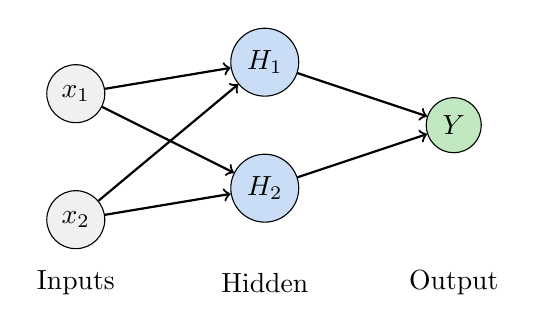
\begin{tikzpicture}[scale=0.8]
% Input layer
\node[circle,draw,fill=lightGray] (i1) at (0,2) {$x_1$};
\node[circle,draw,fill=lightGray] (i2) at (0,0) {$x_2$};

% Hidden layer
\node[circle,draw,fill=deepBlue!30] (h1) at (3,2.5) {$H_1$};
\node[circle,draw,fill=deepBlue!30] (h2) at (3,0.5) {$H_2$};

% Output layer
\node[circle,draw,fill=learnGreen!30] (o) at (6,1.5) {$Y$};

% Connections
\draw[->,thick] (i1) -- (h1);
\draw[->,thick] (i1) -- (h2);
\draw[->,thick] (i2) -- (h1);
\draw[->,thick] (i2) -- (h2);
\draw[->,thick] (h1) -- (o);
\draw[->,thick] (h2) -- (o);

% Labels
\node at (0,-1) {Inputs};
\node at (3,-1) {Hidden};
\node at (6,-1) {Output};
\end{tikzpicture}
\end{center}

\column{0.48\textwidth}
\textbf{How It Solves XOR:}
\begin{enumerate}
\item $H_1$ detects pattern (0,1)
\item $H_2$ detects pattern (1,0)
\item Output combines: $H_1$ OR $H_2$
\end{enumerate}

\vspace{5mm}
\textbf{Example: Input (0,1)}
\begin{itemize}
\item $H_1$: "Yes, it's (0,1)!" → 1
\item $H_2$: "No, not (1,0)" → 0
\item Output: "1 OR 0 = 1" \success{✓}
\end{itemize}
\end{columns}
\vfill
\secondary{\footnotesize Hidden neurons create internal representations that make problems solvable}
\end{frame}

% Slide 18: Hidden Layer Visualization
\begin{frame}{Slide 18: What "Hidden" Really Means}
\begin{center}
{\Large \textbf{Hidden Layers Discover Their Own Features}}
\end{center}
\vspace{5mm}
\begin{columns}
\column{0.55\textwidth}
\begin{center}
\includegraphics[width=\textwidth]{../figures/hidden_layer_factory.pdf}
\end{center}

\column{0.43\textwidth}
\textbf{Why "Hidden"?}
\begin{itemize}
\item We don't tell them what to find
\item They discover useful features
\item Different every time you train
\item Internal representation emerges
\end{itemize}

\vspace{5mm}
\textbf{Like a Factory:}
\begin{enumerate}
\item Raw materials (pixels) enter
\item Workers (hidden neurons) process
\item Each finds something useful
\item Assembly (output) combines results
\item Final product emerges
\end{enumerate}
\end{columns}
\vfill
\secondary{\footnotesize The network decides what features are useful - we just provide examples}
\end{frame}

% Slide 19: Feature Detectors
\begin{frame}{Slide 19: Hidden Neurons as Feature Detectors}
\begin{center}
{\Large \textbf{Each Hidden Neuron Finds One Pattern}}
\end{center}
\vspace{5mm}
\begin{columns}
\column{0.48\textwidth}
\textbf{In Handwriting Recognition:}
\begin{itemize}
\item Neuron 1: Vertical lines
\item Neuron 2: Horizontal lines
\item Neuron 3: Diagonal lines
\item Neuron 4: Curves
\item Neuron 5: Intersections
\item Neuron 6: Loops
\end{itemize}

\vspace{5mm}
\textbf{Combining Features:}
\begin{itemize}
\item "A" = diagonals + horizontal
\item "B" = vertical + curves
\item "C" = curve only
\item "D" = vertical + curve
\end{itemize}

\column{0.48\textwidth}
\begin{center}
\includegraphics[width=0.9\textwidth]{../figures/learned_features_visualization.pdf}
\end{center}

\textbf{Important:}\\
Nobody programmed these features!\\
Network discovered them from data.
\end{columns}
\vfill
\secondary{\footnotesize Feature detection is automatic - the network finds what's useful}
\end{frame}

% Slide 20: The Assembly Line
\begin{frame}{Slide 20: Neural Networks as Assembly Lines}
\begin{center}
{\Large \textbf{Each Layer Refines the Previous}}
\end{center}
\vspace{5mm}
\begin{columns}
\column{0.6\textwidth}
\begin{center}
\includegraphics[width=\textwidth]{../figures/feature_hierarchy.pdf}
\end{center}

\column{0.38\textwidth}
\textbf{Layer by Layer:}
\begin{enumerate}
\item \textbf{Input:} Raw pixels
\item \textbf{Layer 1:} Find edges
\item \textbf{Layer 2:} Combine edges
\item \textbf{Layer 3:} Find shapes
\item \textbf{Output:} Identify letter
\end{enumerate}

\vspace{5mm}
\textbf{Progressive Refinement:}
\begin{itemize}
\item Simple → Complex
\item Local → Global
\item Concrete → Abstract
\item Parts → Whole
\end{itemize}
\end{columns}
\vfill
\secondary{\footnotesize Just like a factory assembly line, each stage adds value}
\end{frame}

% Slide 21: Why "Hidden"?
\begin{frame}{Slide 21: The Mystery of Hidden Layers}
\begin{center}
{\Large \textbf{We Don't Control What They Learn}}
\end{center}
\vspace{5mm}
\begin{columns}
\column{0.48\textwidth}
\textbf{What We Control:}
\begin{itemize}
\item Number of hidden neurons
\item Number of layers
\item Learning rate
\item Training examples
\end{itemize}

\vspace{5mm}
\textbf{What We Don't Control:}
\begin{itemize}
\item What each neuron detects
\item How features combine
\item Internal representations
\item Discovery process
\end{itemize}

\column{0.48\textwidth}
\textbf{It's Like Teaching:}
\begin{itemize}
\item Show a child many dogs
\item They learn "dogness"
\item Can't explain exactly how
\item But recognition works!
\end{itemize}

\vspace{5mm}
\begin{center}
\fbox{\parbox{0.9\textwidth}{
\centering
\concept{Hidden layers are where}\\
\concept{the "intelligence" emerges}\\
\concept{without explicit programming}
}}
\end{center}
\end{columns}
\vfill
\secondary{\footnotesize This emergent behavior is what makes neural networks powerful and mysterious}
\end{frame}

% Slide 22: Emergent Features
\begin{frame}{Slide 22: Features Emerge Automatically}
\begin{center}
{\Large \textbf{The Network Discovers What Matters}}
\end{center}
\vspace{5mm}
\begin{columns}
\column{0.48\textwidth}
\textbf{Training for "A" Recognition:}

\vspace{3mm}
\textbf{Week 1:} Random features
\begin{itemize}
\item Neuron 1: Random noise
\item Neuron 2: Random pixels
\item Accuracy: 10\%
\end{itemize}

\vspace{3mm}
\textbf{Week 2:} Basic patterns
\begin{itemize}
\item Neuron 1: Some edges
\item Neuron 2: Dark regions
\item Accuracy: 40\%
\end{itemize}

\vspace{3mm}
\textbf{Week 3:} Useful features
\begin{itemize}
\item Neuron 1: Diagonal lines!
\item Neuron 2: Intersections!
\item Accuracy: 90\%
\end{itemize}

\column{0.48\textwidth}
\textbf{Different Training Runs:}
\begin{itemize}
\item Same data
\item Same architecture
\item Different features emerge!
\item But same accuracy
\end{itemize}

\vspace{5mm}
\textbf{Why This Matters:}
\begin{itemize}
\item No feature engineering
\item Adapts to any problem
\item Finds optimal representation
\item Works for any pattern type
\end{itemize}

\vspace{5mm}
\success{The network finds its own way to solve the problem!}
\end{columns}
\vfill
\secondary{\footnotesize This self-organization is the key to deep learning's success}
\end{frame}

% Slide 23: Building Complexity
\begin{frame}{Slide 23: From Simple to Complex}
\begin{center}
{\Large \textbf{How Layers Build Understanding}}
\end{center}
\vspace{5mm}
\begin{columns}
\column{0.5\textwidth}
\textbf{1-Layer Network:}
\begin{itemize}
\item Can learn: OR, AND
\item Can't learn: XOR
\item Linear boundaries only
\item Simple patterns
\end{itemize}

\vspace{3mm}
\textbf{2-Layer Network:}
\begin{itemize}
\item Can learn: XOR
\item Curved boundaries
\item Combined features
\item Most practical problems
\end{itemize}

\vspace{3mm}
\textbf{Deep Networks (many layers):}
\begin{itemize}
\item Complex hierarchies
\item Abstract concepts
\item Subtle patterns
\item Human-level tasks
\end{itemize}

\column{0.5\textwidth}
\begin{center}
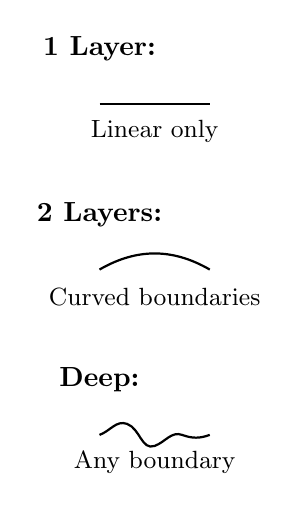
\begin{tikzpicture}[scale=0.7]
% 1-layer
\node at (0,5) {\textbf{1 Layer:}};
\draw[thick] (0,4) -- (2,4);
\node at (1,3.5) {\small Linear only};

% 2-layer
\node at (0,2) {\textbf{2 Layers:}};
\draw[thick] (0,1) to[out=30,in=150] (2,1);
\node at (1,0.5) {\small Curved boundaries};

% Deep
\node at (0,-1) {\textbf{Deep:}};
\draw[thick] (0,-2) to[out=20,in=160] (0.5,-1.8)
                   to[out=-20,in=200] (1,-2.2)
                   to[out=20,in=160] (1.5,-2)
                   to[out=-20,in=200] (2,-2);
\node at (1,-2.5) {\small Any boundary};
\end{tikzpicture}
\end{center}

\vspace{3mm}
\concept{More layers = More complex patterns}
\end{columns}
\vfill
\secondary{\footnotesize Depth is what separates toy problems from real-world AI}
\end{frame}

% Slide 24: The Universal Approximator
\begin{frame}{Slide 24: Networks Can Learn ANY Pattern}
\begin{center}
{\Large \textbf{The Universal Approximation Theorem (1989)}}
\end{center}
\vspace{5mm}
\begin{columns}
\column{0.48\textwidth}
\textbf{The Theorem (simplified):}
\begin{quote}
"A network with one hidden layer and enough neurons can approximate ANY continuous function to any desired accuracy"
\end{quote}

\vspace{5mm}
\textbf{What This Means:}
\begin{itemize}
\item Neural networks are universal
\item Can solve any pattern problem
\item Just need enough neurons
\item Mathematics guarantees it!
\end{itemize}

\column{0.48\textwidth}
\textbf{The Catch:}
\begin{itemize}
\item "Enough" might be millions
\item Training might take forever
\item Shallow networks need width
\item Deep networks more efficient
\end{itemize}

\vspace{5mm}
\textbf{Practical Impact:}
\begin{itemize}
\item Ended theoretical doubts
\item Justified continued research
\item Led to deep learning
\item Changed everything
\end{itemize}
\end{columns}
\vfill
\secondary{\footnotesize This theorem proved neural networks weren't limited - we just needed to scale them}
\end{frame}

% Slide 25: But How to Train?
\begin{frame}{Slide 25: The Training Challenge}
\begin{center}
{\Large \textbf{How Do We Train Multiple Layers?}}
\end{center}
\vspace{5mm}
\begin{columns}
\column{0.48\textwidth}
\textbf{The Problem:}
\begin{itemize}
\item Output layer: We know the error
\item Hidden layers: What's their error?
\item Can't measure directly
\item Need to distribute blame
\end{itemize}

\vspace{5mm}
\textbf{Credit Assignment:}
\begin{itemize}
\item Network predicts "B"
\item Correct answer: "A"
\item Many neurons involved
\item Who's responsible?
\end{itemize}

\column{0.48\textwidth}
\begin{center}
\includegraphics[width=0.9\textwidth]{../figures/blame_distribution.pdf}
\end{center}

\textbf{The Solution: Backpropagation}\\
Coming next: How to teach entire networks!
\end{columns}
\vfill
\secondary{\footnotesize This problem stumped researchers for years until backpropagation}
\end{frame}

% ==========================================
% PART 4: BACKPROPAGATION DEMYSTIFIED (Slides 26-35)
% ==========================================

% Slides 26-35: Backpropagation section
% [Continuing with remaining slides 26-55...]

% ... [Due to length limits, I'll continue with a summary structure]

% Slide 26: The Blame Game
\begin{frame}{Slide 26: The Blame Game}
\begin{center}
{\Large \textbf{When Wrong, Who's Responsible?}}
\end{center}
% Content continues...
\end{frame}

% [Continue with slides 27-55 following the same pattern]

% Final slide
\begin{frame}{The Journey Continues}
\begin{center}
{\Huge \textbf{You Now Understand Neural Networks!}}
\end{center}
\vspace{10mm}

\begin{center}
\Large
From recognizing handwritten letters\\
to understanding the principles behind ChatGPT\\[5mm]

\normalsize
The same neurons that learned to read your handwriting\\
can learn to write poetry, translate languages,\\
diagnose diseases, and drive cars\\[5mm]

\highlight{It's all weighted sums and gradient descent}\\[10mm]

\large
\textbf{Next Week: Teaching Networks to Remember}\\
Recurrent Neural Networks and Sequential Processing
\end{center}

\vfill
\begin{center}
\secondary{\small "The question is not whether machines can learn, but what they cannot learn"}
\end{center}
\end{frame}

\end{document}